Having established on synthetic universes that the prior-consistent estimators of Section~\ref{sec:estimators} are calibrated where the bare-Gaussian kernel is not (Section~\ref{sec:coverage}), we now turn to the configuration that motivated this work: a simulated EMRI detection campaign evaluated against the real GLADE+ galaxy catalogue \citep{Dalya:2021ewn}. We emphasize at the outset that the events are simulated; every statement in this section concerns estimator calibration at the injected truth $h = 0.73$, not a measurement of the Hubble constant in nature.

\subsection{The seed600 campaign on GLADE+}

The event sample (internally, the \textit{seed600} catalogue) comprises 3375 detected EMRI events drawn from the population model at injected $h = 0.73$, each carrying a Fisher-matrix (Cram\'er--Rao) covariance and a measurement realization drawn from the corresponding multivariate normal. % src: results/commission_20260701/redteam/crux_realdata.md
A quality cut requiring a relative luminosity-distance uncertainty below $0.1$ retains 3355 events. % src: results/commission_20260701/redteam/crux_realdata.md
Hosts are matched against the reduced GLADE+ catalogue, which after pruning to galaxies with finite black-hole-mass proxies contains $9\,060\,017$ galaxies with $z \in [0.003, 1.33]$.\footnote{The runs reported here used a column-aligned reconstruction of the reduced-catalogue schema that preserves the science columns (positions, redshifts, redshift uncertainties, and mass proxies) byte-for-byte; the two padding columns it introduces are not consumed by the likelihood. % src: results/commission_20260701/redteam/crux_realdata.md
} % src: results/commission_20260701/redteam/crux_realdata.md
The selection function $p_\mathrm{det}$ is estimated from a dedicated injection campaign of $72\,000$ events at $h = 0.73$, binned in six equal-$|\sin\beta|$ sky bands, where $\beta$ denotes the ecliptic latitude (unrelated to the selection normalizations $\beta_G$, $\beta_{\bar G}$); all 3355 analysis events fall inside the resulting $p_\mathrm{det}$ grid. % src: results/commission_20260701/redteam/crux_realdata.md
At the injected truth the in-catalogue partition weight is $w_G = \beta_G/D(h) = 0.8175$. % src: results/commission_20260701/redteam/crux_realdata.md

One caveat about the event sample must be stated here. The seed600 catalogue was selected at the pre-correction signal-to-noise scale of the simulation pipeline, before the missing $\mathrm{d}t^2$ discrete-to-continuous Fourier normalization in the inner product was repaired (Section~\ref{sec:budget}): the code-level signal-to-noise ratio was the physical one divided by ten, so the nominal detection threshold of 20 in fact selected a physical-SNR~$\geq 200$ population with depth $z \lesssim 0.11$ rather than the $z \lesssim 1.5$ reach of a true threshold-20 sample, and the accompanying Fisher uncertainties are ten times too pessimistic for such loud events. % src: .planning/gate/G8_inner_product_finding.md; .planning/gate/G7_systematics_budget.md (row 1)
Because the identical (mis-scaled but internally consistent) inner product enters both the event selection and the injection campaign that defines $p_\mathrm{det}$, the dataset remains a self-consistent mock universe, and the de-rail comparison below --- identical data, identical events, identical catalogue, only the estimator changed --- is unaffected. % src: .planning/gate/GATE_SIGNOFF.md (queued confirmation "scientifically valid for the de-rail claim")
Forecast-grade constraints require post-fix re-simulation and are deferred to Paper~B.

\subsection{The de-rail matrix}

The demonstration holds the data fixed and swaps only the normalization of the likelihood. For computational economy --- a single production evaluation is dispatch-bound at roughly five minutes per $h$ value --- the matrix uses a 494-event subsample of seed600 on a seven-point grid $h \in \{0.60, 0.65, 0.70, 0.73, 0.76, 0.80, 0.86\}$, combining events with a flat prior by summing per-event log-likelihoods and normalizing over the grid. % src: results/commission_20260701/redteam/crux_realdata.md
Table~\ref{tab:derail} and Fig.~\ref{fig:derail} give the result; we call a posterior \textit{railed} when essentially all of its mass sits on a grid endpoint (edge mass $\approx 1$).

\begin{table}
\centering
\caption{De-rail matrix on identical real GLADE+ data (494-event seed600 subsample, injected $h = 0.73$, seven-point grid $[0.60, 0.86]$). ``Bare'' and ``volume'' denote the host-redshift kernel of Sections~\ref{sec:pitfall} and~\ref{sec:estimators}; the denominator column distinguishes the global single-ratio normalization from the local per-event ratio-of-sums. Edge mass is the posterior mass on the nearest grid endpoint.}
\label{tab:derail}
\begin{tabular}{lllccc}
\hline
Configuration & Kernel & Denom. & MAP & Mean & Edge mass \\
\hline
Production (pre-fix) & bare & global & $0.86$ & $0.860$ & $1.0$ \\ % src: results/commission_20260701/redteam/crux_results.json (prod)
$1/(4\pi)$ only & bare & global & $0.60$ & $0.600$ & $1.0$ \\ % src: results/commission_20260701/redteam/derail_matrix_results.json (prod_global)
Volume, global & volume & global & $0.76$ & $0.755$ & $2.3\times10^{-2}$ \\ % src: .planning/gate/G3_ablation_cube.json (volume_global)
Local ratio & bare & local & $0.73$ & $0.730$ & $1.8\times10^{-12}$ \\ % src: results/commission_20260701/redteam/derail_matrix_results.json (local_ratio)
Volume deconv. & volume & local & $0.73$ & $0.740$ & $2.9\times10^{-4}$ \\ % src: results/commission_20260701/redteam/derail_matrix_results.json (volume_deconv)
Catalogue only & bare & local & $0.73$ & $0.737$ & $3.7\times10^{-5}$ \\ % src: results/commission_20260701/redteam/crux_results.json (catonly)
\hline
\end{tabular}
\end{table}

\begin{figure}
\centering
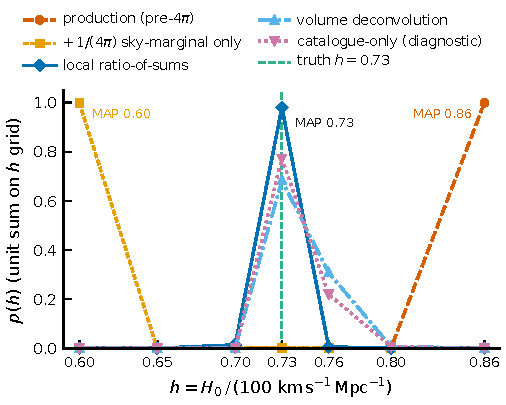
\includegraphics[width=\columnwidth]{figures/fig_derail_matrix.pdf}
\caption{De-railing the GLADE+ posterior. Posterior probability over the seven-point $h$ grid for the de-rail progression of Table~\ref{tab:derail}, on identical data (494-event seed600 subsample, injected truth $h = 0.73$). The pre-fix production estimator rails at the upper grid edge ($h = 0.86$, edge mass $1.0$); applying only the isotropic $1/(4\pi)$ completion sky marginal flips the rail to the lower edge ($h = 0.60$); either prior-consistent normalization --- the local ratio-of-sums or the volume-deconvolved kernel --- yields an interior posterior peaked at the injected value ($98$ per cent and $68$ per cent of the mass at $h = 0.73$, respectively). % src: results/commission_20260701/redteam/derail_matrix_results.json; results/commission_20260701/redteam/crux_results.json
}
\label{fig:derail}
\end{figure}

The progression reads as follows. The pre-fix production estimator --- bare-Gaussian host-$z$ kernel, global denominator, and the completion-term sky factor evaluated at its peak density --- piles $100$ per cent of the posterior mass on the upper grid edge, $\mathrm{MAP} = 0.86$; the archived production run on the full 3375-event sample rails at the same edge. % src: results/commission_20260701/redteam/crux_results.json; results/commission_20260701/redteam/crux_realdata.md
Replacing the peak-density sky factor by the correct isotropic $1/(4\pi)$ marginal (Section~\ref{sec:pitfall}; Appendix~\ref{sec:app:sky}) removes a completion term inflated by a factor of order $1640$ --- and the posterior rails again, now at the \emph{lower} edge, $\mathrm{MAP} = 0.60$ with edge mass $1.0$. % src: results/commission_20260701/redteam/crux_realdata.md (~1640x); results/commission_20260701/redteam/derail_matrix_results.json (prod_global)
This sign flip is exactly the behaviour anticipated by the mechanism analysis of Section~\ref{sec:pitfall}: the sky fix is necessary but not sufficient, because it exposes the still-inconsistent in-catalogue normalization underneath. Since both railed modes sit on grid endpoints, the unconstrained maxima of those posteriors may lie outside $[0.60, 0.86]$ altogether; the rail location is a property of the grid, not of the data.

Either prior-consistent repair then de-rails the posterior. The local ratio-of-sums normalization (Section~\ref{sec:estimators}) yields an interior peak at the injected value, $\mathrm{MAP} = 0.73$ with $98$ per cent of the mass on that grid point and edge mass $\sim 10^{-12}$. % src: results/commission_20260701/redteam/derail_matrix_results.json (local_ratio)
The volume-deconvolved kernel on top of the local ratio gives $\mathrm{MAP} = 0.73$ as well, with $68$ per cent of the mass at $0.73$ and $31$ per cent at $0.76$. % src: results/commission_20260701/redteam/derail_matrix_results.json (volume_deconv)
The catalogue-only baseline, which discards the completion term entirely, was never railed: it peaks at $0.73$ with $77$ per cent of the mass there and $22$ per cent at $0.76$. % src: results/commission_20260701/redteam/crux_results.json (catonly)
The in-catalogue information was present all along; the rail is manufactured by the completion-term normalization, not by photometric-redshift information starvation (Section~\ref{sec:postmortem}). This is worth stressing because on these data the completion machinery, not the host matches, carries most of the constraint: for 3331 of the 3355 events the in-catalogue completion numerator evaluates to zero at working precision (more than 5 per cent of the quadrature weight falls outside the $p_\mathrm{det}$ grid), yet every per-event likelihood remains finite and positive --- so a mis-normalized completion term is multiplied coherently across essentially the whole sample. % src: results/commission_20260701/redteam/crux_realdata.md

\subsection{Two-factor ablation}

The two repairs act on different defects, and their contributions separate cleanly. Fig.~\ref{fig:ablation} shows the ablation cube: starting from the railed $1/(4\pi)$-only configuration ($\mathrm{MAP} = 0.60$), installing the volume kernel consistently in \emph{both} the per-event numerator and its selection denominator --- while retaining the global denominator --- already de-rails the posterior, moving it to an interior $\mathrm{MAP} = 0.76$ (mean $0.755$, edge mass $2.3\times10^{-2}$). % src: .planning/gate/G3_ablation_cube.json (volume_global)
Replacing the global denominator by the local per-event ratio then removes the remaining $+0.03$ displacement, landing on $\mathrm{MAP} = 0.73$. % src: .planning/gate/G3_ablation_cube.json; .planning/gate/GATE_SIGNOFF.md (G3 row)
Kernel consistency is therefore the de-railing factor, while the global-versus-local denominator choice controls the residual offset --- consistent with the $h$-dependent tilt of the global normalization quantified in Appendix~\ref{sec:app:betag}.

\begin{figure}
\centering
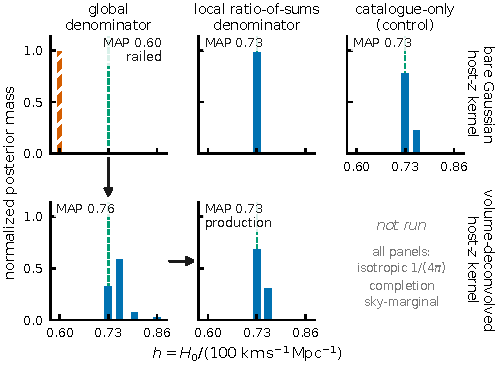
\includegraphics[width=\columnwidth]{figures/fig_ablation.pdf}
\caption{Two-factor ablation on the same 494-event GLADE+ sample, varying one estimator factor at a time. With the global denominator retained, moving the bare kernel to the prior-consistent volume kernel de-rails the posterior from the $h = 0.60$ edge to an interior $\mathrm{MAP} = 0.76$; switching the global denominator to the local ratio-of-sums removes the remaining $+0.03$ offset, giving $\mathrm{MAP} = 0.73$ (mean $0.740$ with, or $0.730$ without, the volume deconvolution). % src: .planning/gate/G3_ablation_cube.json
}
\label{fig:ablation}
\end{figure}

Finally, the $+0.010$ offset between the two cured estimators (means $0.740$ versus $0.730$) matches in sign, and roughly in magnitude, the Eddington-type debiasing that the volume prior was measured to provide on synthetic universes (Section~\ref{sec:coverage}): the bare-Gaussian kernel biases the numerator low, and the deconvolution removes that bias. % src: results/commission_20260701/redteam/derail_matrix_results.json; results/commission_20260701/redteam/crux_realdata.md
The real-data shift is smaller than the $2$--$3$ per cent measured synthetically at $\sigma_z \simeq 0.035$ because most GLADE+ hosts in this sample carry near-spectroscopic redshift uncertainties. % src: results/commission_20260701/redteam/crux_realdata.md

The matrix above rests on the 494-event subsample and its coarse seven-point grid. A full-scale confirmation --- the production pipeline with the volume-deconvolved default applied to all 3375 seed600 events over the complete 38-value grid spanning $[0.60, 0.86]$ --- is running on the compute cluster at the time of writing, and its posterior maximum is $\text{[PENDING]}$. % [RESULT PENDING: cluster jobs 5698617/5698618 (38-task eval array + dependent combine) provide the full-grid volume_deconv combined posterior MAP; expected peaked ~0.73] % src: .planning/HANDOFF-DERAIL-CLUSTER-CONFIRM-20260702.md
